%%%%%%%%%%%%%%%%%%%%%%%%%%%%%%%%%%%%%%%%%%%%%%%%%%%%%%%
%%%%%   ARCHIVO PRINCIPAL DEL ANTEPROYECTO         %%%%
%%%%%%%%%%%%%%%%%%%%%%%%%%%%%%%%%%%%%%%%%%%%%%%%%%%%%%%
\documentclass[12pt,letterpaper,spanish]{article}
\usepackage[T1]{fontenc}
\usepackage[utf8,latin1]{inputenc}
\usepackage[spanish,activeacute]{babel}
\usepackage{anysize}
\usepackage[pdftex]{graphicx}
\usepackage{pdfpages}
\marginsize{3cm}{3cm}{2cm}{2cm}
 % Set equal margins on book style
%\setlength{\oddsidemargin}{30pt}
%\setlength{\evensidemargin}{30pt}
%\setlength{\marginparwidth}{30pt}
%\setlength{\footskip}{30pt}
\makeindex
%\linespread{1.5}
\graphicspath{{images/}}

%%%%%%%%%%%%%%%%%%%%%%%%%%%%%%%%%%%%%%%%%%%%%%%%%%%%%%%%%%%%%%%%%%%%%%
%%% Mise en page
%%%%%%%%%%%%%%%%%%%%%%%%%%%%%%%%%%%%%%%%%%%%%%%%%%%%%%%%%%%%%%%%%%%%%

%%%%%%%%%%%%%%%%%%%%%%%%%%%%%%%%%%%%%%%%%%%%%%%%%%%%%%%%%%%%%%%%%%%%%%

% pour les couples de quelque chose

\newcommand{\lan}{\ensuremath{\langle\,}}
\newcommand{\ran}{\ensuremath{\,\rangle}}

% Retouche de l'environnement tabbing
\makeatletter

\def\@tabreset{\global\@nxttabmar\@firsttab\global\advance\@nxttabmar\@ne}
\def\tabbing{\lineskip \z@\let\>\@rtab\let\<\@ltab\let\=\@settab
     \let\+\@tabplus\let\-\@tabminus\let\'\@tabrj\let\0\@tabreset
     \let\\=\@tabcr
     \global\@hightab\@firsttab
     \global\@nxttabmar\@firsttab
     \dimen\@firsttab\@totalleftmargin
     \global\@tabpush \global\@rjfieldfalse
     \trivlist \item[]\if@minipage\else\vskip\parskip\fi
     \setbox\@tabfbox\hbox{\rlap{\indent\hskip\@totalleftmargin
      \the\everypar}}\def\@itemfudge{\box\@tabfbox}\@startline\ignorespaces}

% d�finition de l'environnement langage : ne pas decaler le texte

\newenvironment{lang}{\small \begin{tt}%
\begin{tabbing}xx\=xx\=xx\=xx\=xx\=xx\=xx\=xx\=xx\=xx\=xx\=xx\=xx\=\+\kill}%
{\end{tabbing}\end{tt}\ignorespaces}


\newenvironment{langscript}{\scriptsize \begin{tt}%
\begin{tabbing}xx\=xx\=xx\=xx\=xx\=xx\=xx\=xx\=xx\=xx\=xx\=xx\=xx\=\+\kill}%
{\end{tabbing}\end{tt}\ignorespaces}

% 
%	commentaires cadr�s a droite et normaux
%
\newlength{\comml}
\def\commp#1{\@stopfield\@addfield\comml\linewidth
\global\advance\comml -\wd\@curline
\global\advance\comml -\dimen\@curtabmar
\@startfield\parbox[t]{\comml}{\normalfont\it /* #1 */}}
\newcommand{\comm}[1]{\normalfont\it /* #1 */}

\newcommand{\prodi}{{\Large$\ast$}$_\cap$\xspace}
\newcommand{\prode}{{\Large$\ast$}$_\cup$\xspace}
\newcommand{\restif}{\ensuremath{\Gamma_{\text{si}}}\xspace}
\newcommand{\restin}{\ensuremath{\Gamma_{\text{en}}}\xspace}
\newcommand{\fleche}{\ensuremath{\rightarrow}\xspace}

% environnements Definition, Algorithme, Requete, �pigraphe
% cambie al ingles los nombres

\makeatother
\newcounter{CptDefinition}
\renewcommand{\theCptDefinition}{Definici�n \arabic{CptDefinition}}
\newlength{\monparindent}
\newenvironment{mydefinition}[1]{\setlength{\monparindent}{\parindent}%
              \setlength{\parindent}{0pt}%
              \refstepcounter{CptDefinition}%
              \par\vspace{.3\baselineskip}\noindent{\bf
                              \theCptDefinition} ({\bf #1})\\ \it}
                              \\
                              %{\\{\small $\square$}%                   		
                              % \setlength{\parindent}{\monparindent}%
                              % \vspace{.3\baselineskip}\par\ignorespaces}

\newcounter{CptOperator}
\renewcommand{\theCptOperator}{Funci�n \arabic{CptOperator}}
%\newlength{\monparindent}
\newenvironment{operator}[1]{\setlength{\monparindent}{\parindent}%
              \setlength{\parindent}{0pt}%
              \refstepcounter{CptOperator}%
              \par\vspace{.3\baselineskip}\noindent{\bf
                              \theCptOperator} ({\bf #1})\\ \it}
                              \\
                              %{{\small $\square$}%
                              % \setlength{\parindent}{\monparindent}%
                              % \vspace{.3\baselineskip}\par\ignorespaces}



\newcounter{CptAlgorithme}
\renewcommand{\theCptAlgorithme}{Algorithm \arabic{CptAlgorithme}}
\newenvironment{algorithme}[1]{\refstepcounter{CptAlgorithme}%
                               \par\noindent{\bf \theCptAlgorithme}~: %
                             {\em #1 \newline\ignorespaces}}%
                           {\par\ignorespaces}

\newcounter{CptRequete}
\renewcommand{\theCptRequete}{Q\arabic{CptRequete}}
\newcommand{\requete}[2]{\refstepcounter{CptRequete}%
                               \par\noindent{\bf \theCptRequete}~: %

\ifthenelse{\equal{#1}{}}{}{{\bf #1 \newline}}%
{\em #2\par\vspace{-1mm}\ignorespaces}}

\newcommand{\reqavecref}[3]{\par\noindent{\bf \ref{#1}}~: %
\ifthenelse{\equal{#2}{}}{}{{\bf #2 \newline}}%
{\em #3\par\vspace{-1mm}\ignorespaces}}

\newcommand{\epigraphe}[2]{%
\begin{flushright}%
\begin{minipage}{0.35\textwidth}%
%#1\par%

\vspace{0.5\baselineskip}%
\raggedleft{#2}%
\par
\end{minipage}%
\end{flushright}%
}

% pour les fonctions d'expansion et d'approximation sur les granules:

\newcommand{\expand}[1]{%
\ensuremath{\text{\Large$\epsilon_{\text{\scriptsize #1}}$}}}
\newcommand{\approxi}[1]{%
\ensuremath{\text{\Large$\alpha_{\text{\scriptsize #1}}$}}}

\newcommand{\la}[1]{\textsf{#1}}
\newcommand{\sub}[2]{#1$_{\text{#2}}$}
\newcommand{\lasub}[2]{\la{#1$_{\text{#2}}$}}
\newcommand{\textul}[1]{\ensuremath{\underline{\text{#1}}}}

\newcommand{\malambda}[2]{\ensuremath{\lambda}\mbox{#1 {\tiny $\bullet$}} #2}

% mes environnements itemize

\newenvironment{suite}{\begin{list}{$\bullet$}{%
           \setlength{\itemsep}{\parsep}%
           \setlength{\partopsep}{0pt}}}%
           {\end{list}}
\newenvironment{suite2}{\begin{list}{--}{%
           \setlength{\itemsep}{0pt}%
           \setlength{\parsep}{0pt}%
           \setlength{\partopsep}{-1pt}}}%
           {\end{list}}

% mon environnement figure

\newenvironment{figure-centree}{\begin{figure}[hbt] \begin{center}}%
                               {\end{center}\end{figure}}

% pour d�finir la s�mantique de OQLiST

\newcommand{\vv}[2]{\ensuremath{{[\![\,\text{#1}]\!]}\,_{%
\ifthenelse{\equal{#2}{}}{\nu}{#2}}}}

\newcommand{\semantique}[1]{%
%\begin{center}%
%\fbox{
%\begin{minipage}{\textwidth}%
%\vspace*{-4mm}%
\begin{tabbing}%
#1%
\end{tabbing}
%\vspace*{-4mm}
%\end{minipage}%}
%\vspace*{5mm}%
%\end{center}%
\par\ignorespaces}%
\newcommand{\typage}[2]{
\ensuremath{\displaystyle \text{Typage~: }%
\frac{\mathrm{#1}}{\mathrm{#2}}}}


%%%%%%%%%%%%%%%%%%%%%%%%%%%%

% pour eviter les orphelins
%%%% debut macro %%%%
\widowpenalty=10000
\clubpenalty=10000
\raggedbottom
%%%% fin macro %%%%

\newtheorem{predef}{Definition}
\newtheorem{preexample}{Example}

%\newenvironment{definition}[1]%
%    {\begin{predef}[#1]\it}{\end{predef}}

%\newenvironment{example}%
%    {\begin{preexample}\it}{\end{preexample}}


\newenvironment{mdexpr}%
    {\begin{quote}}{\end{quote}}

%%%%% mes figures %%%%%%%%%%%%

\newcommand{\fig}[3]{
\begin{figure}[hbt!]
\vspace*{.2in}
\centerline{\includegraphics[scale=#2]{figs/#1}}
\caption{#3}
\vspace*{.2in}
\label{#1}
\end{figure} }

\newcommand{\figp}[3]{
\begin{figure}[p]
\vspace*{.2in}
\centerline{\includegraphics[scale=#2]{figs/#1}}
\caption{#3}
\vspace*{.2in}
\label{#1}
\end{figure} }


\newcommand{\figppt}[3]{
\begin{figure}[hbt!]
\vspace*{.2in}
\centerline{\includegraphics[angle=-90,scale=#2]{figs/#1}}
\caption{#3}
\vspace*{.2in}
\label{#1}
\end{figure} }



%%%%% mes commandes %%%%%%%%%%%%

\newcommand{\dimtemps}{{\sl Temps} }

\newcommand{\dimt}{{\sl Temps}}
\newcommand{\njour}{{\sl jour} }
\newcommand{\nj}{{\sl jour}}
\newcommand{\pjourF}{{\sl jourF�ri�}}
\newcommand{\pnomJ}{{\sl nomJour}}

\newcommand{\nmois}{{\sl mois} }
\newcommand{\nm}{{\sl mois}}

\newcommand{\nannee}{{\sl ann�e} }
\newcommand{\nan}{{\sl ann�e}}

\newcommand{\dimmagasin}{{\sl Magasin} }
\newcommand{\dimm}{{\sl Magasin}}

\newcommand{\nville}{{\sl ville} }
\newcommand{\nregion}{{\sl r�gion} }
\newcommand{\npays}{{\sl pays} }

\newcommand{\nv}{{\sl ville}}
\newcommand{\nr}{{\sl r�gion}}
\newcommand{\np}{{\sl pays}}

\newcommand{\dimproduit}{{\sl Produit} }
\newcommand{\dimp}{{\sl Produit}}

\newcommand{\ncode}{{\sl code} }
\newcommand{\nc}{{\sl code}}

\newcommand{\propnom}{{\sl nom} }
\newcommand{\pnom}{{\sl nom}}

\newcommand{\propdesc}{{\sl description} }
\newcommand{\pdesc}{{\sl description}}

\newcommand{\ncategorie}{{\sl cat�gorie} }
\newcommand{\ncat}{{\sl cat�gorie}}

\newcommand{\nrayon}{{\sl rayon} }
\newcommand{\nray}{{\sl rayon}}

\newcommand{\nmarque}{{\sl marque} }

\newcommand{\cubeventes}{{\sl Ventes} }
\newcommand{\cubev}{{\sl Ventes}}

\newcommand{\cubecv}{{\sl Cumul\_Ventes}}

\newcommand{\mquantite}{{\sl quantit�} }
\newcommand{\mquant}{{\sl quantit�}}

\newcommand{\unitesvendues}{{\sl unit�s\_vendues} }
\newcommand{\uvendues}{{\sl unit�s\_vendues}}


\newcommand{\mprix}{{\sl prix} }
\newcommand{\mpr}{{\sl prix}}

\newcommand{\dimdist}{{\sl Distribution} }
\newcommand{\dimd}{{\sl Distribution}}


\newcommand{\ordre}{ $\prec$ }
\newcommand{\ord}{\prec}

\newcommand{\pordre}{ $\preceq^{*}$ }
\newcommand{\pord}{\preceq^{*}}

\newcommand{\toplevel}{$\top$ }
\newcommand{\stoplevel}{$\top$}
\newcommand{\topl}{\top}

\newcommand{\bottomlevel}{$l_{\bot}$ }
\newcommand{\botl}{l_\bot}

\newcommand{\desc}{\rho}
\newcommand{\descr}{ $\rho$ }

\newcommand{\moins}{ \backslash }

\newcommand{\flecheg}{\leftarrow}

\newcommand{\infname}{XXX }
\newcommand{\iname}{XXX}

\newcommand{\comments}[1]{\centerline{#1}}


\newcommand{\sm}{${\cal S}_m$}

\newcommand{\si}{${\cal S}_i$}

\newcommand{\sms}{${\cal S}_m$ }

\newcommand{\sis}{${\cal S}_i$ }

\newcommand{\nomops}{16 }
\newcommand{\nomopsdim}{8 }
\newcommand{\nomopscube}{8 }

\newcommand{\st}{ \vert }



\newcommand{\scatalogue}{{\tt scatalogue}}
\newcommand{\spjaunes}{{\tt spjaunes}}
\newcommand{\sgeog}{{\tt sgeog}}
\newcommand{\sgrenoble}{{\tt sgrenoble}}
\newcommand{\sparis}{{\tt sparis}}
\newcommand{\slondres}{{\tt slondres}}

\newcommand{\sscatalogue}{{\tt scatalogue} }
\newcommand{\sspjaunes}{{\tt spjaunes} }
\newcommand{\ssgeog}{{\tt sgeog} }
\newcommand{\ssgrenoble}{{\tt sgrenoble} }
\newcommand{\ssparis}{{\tt sparis} }
\newcommand{\sslondres}{{\tt slondres} }


\newcommand{\maps}{correspondances }
\newcommand{\map}{correspondance }
\newcommand{\Map}{Correspondance }


\newcommand{\myrule}[3]{
\begin{center}
\begin{minipage}{\textwidth}
%\vspace{-4mm}
\begin{tabbing}
xx\=xx\=xx\=xx\=xx\=xx\=xx\=xx\=xx\=xx\=xx\=xx\=xx\=\+\kill
\> R�gle #1 : \\
\vspace{5mm}
\> \> \> #2 \\
\> \> \> \> \> $\rightarrow$ #3
\end{tabbing}
%\vspace{-4mm}
\end{minipage}
\end{center}
}




\begin{document}
\title{Desempeño de equipos en sistemas colaborativos}
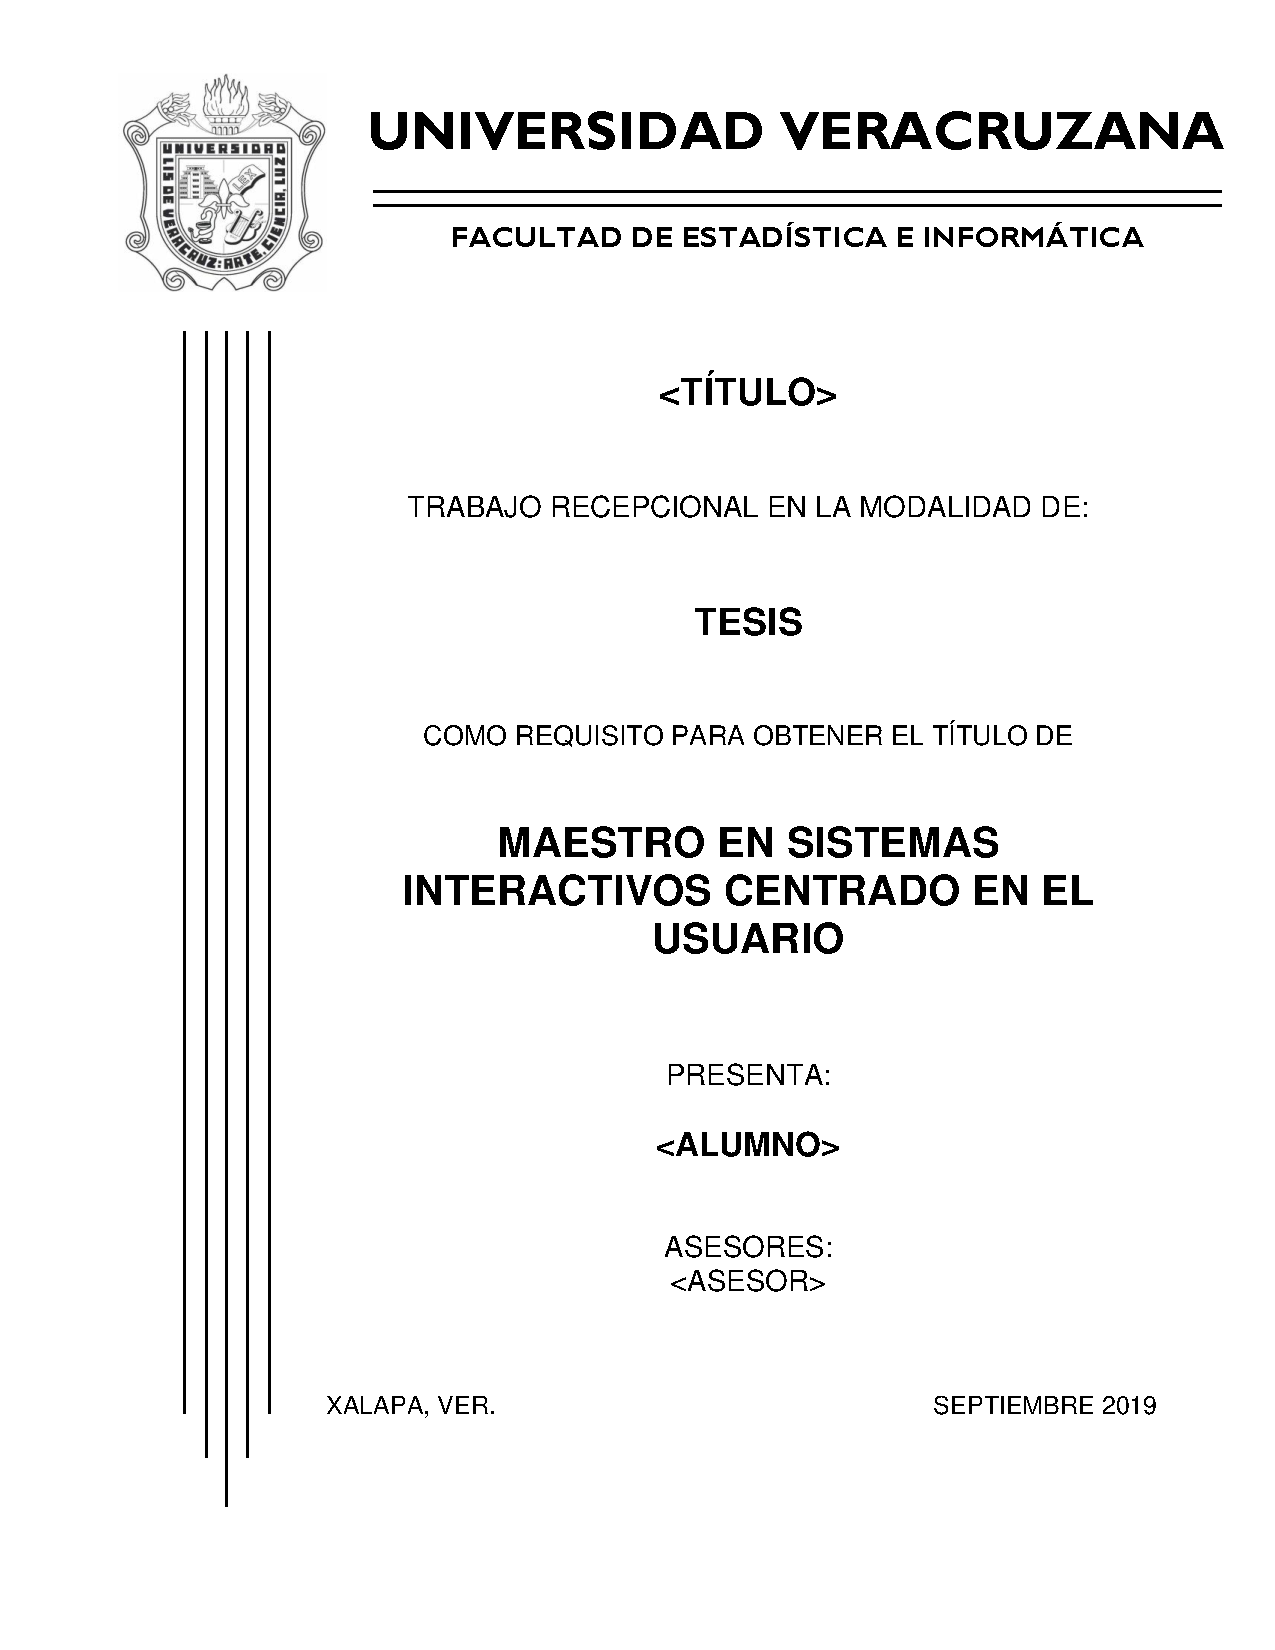
\includepdf{portada.pdf}
%\maketitle
%\thispagestyle{electronic}
%%\newpage
%%M뿯붿rgenes
\marginsize{2.5cm}{2.5cm}{3cm}{3cm}
% Controla los m뿯붿rgenes {izquierda}{derecha}{arriba}{abajo}. 
\tableofcontents
\newpage
%\listoftables
%\listoffigures
%\newpage
%Para las pablabras cortadas
\clubpenalty=10000
\widowpenalty=10000
%Nota: aqu뿯½ podr뿯½as agregar secci뿯½n de abreviaturas.
\section{Introducci�n}

\subsection{Antecedentes}
Los Sistema Colaborativos son sistemas que apoyan a equipos de personas a realizar actividades colaborativas para alcanzar una meta en com�n. Estos sistemas se ven apoyados por el �rea de Visualizaci�n de Informaci�n (VI) para mostrar a los equipos informaci�n gr�fica que derive de datos generados a partir de las interacciones de los usuarios con el entorno. Esta representaci�n visual de datos podr�a apoyar la generaci�n de una consciencia de grupo que pueda ser clave para la toma de decisiones de los integrantes de equipos durante el desarrollo de una actividad colaborativa.

\subsubsection{Sistemas colaborativos}
Los Sistemas Colaborativos (SC) o Groupware derivan del campo de estudio Trabajo Colaborativo Asistido por Computadora (CSCW, por sus siglas en ingl�s), el cual se enfoca en el estudio de grupos de trabajo y busca descubrir c�mo el c�mputo puede apoyarlos. Como �rea de estudio interdisciplinaria, CSCW involucra ciencias sociales (p.ej.psicolog�a, sociolog�a, teor�a organizacional, antropolog�a, entre otras) y ciencias de la computaci�n (p.ej. inteligencia artificial, sistemas distribuidos, dise�o de interfaz de usuario y usabilidad) \cite{Mills2003a}. En el �rea de c�mputo destacan los SC, son sistemas basados en computadora que soportan grupos de gente comprometidos en una tarea com�n (o meta) y que proveen una interfaz para un ambiente compartido \cite{Clarence1991a}.

Los SC consideran los aspectos sociales, pero est�n m�s enfocados en los computacionales: el espacio, tiempo, cantidad de usuarios, entre otros, son interpretados como dimensiones que heredan de los CSCW. Estas dimensiones deben tomarse en cuenta para el dise�o de los SC en aspectos de comunicaci�n, coordinaci�n e interacci�n de usuarios, entre otros, que var�an sus caracter�sticas seg�n la dimensi�n que sea m�s relevante en el SC (p.ej. un SC con comunicaci�n a distancia). 

\subsubsection{Desempe�o de equipos}
El aspecto de interacci�n de usuarios se ocupa de construir y mantener la relaci�n entre los usuarios del SC, administrando la atenci�n o consciencia de las tareas y actividades de un usuario hacia otros; para esto, hace uso de la coordinaci�n y la comunicaci�n \cite{Mills2003a}. A trav�s de la consciencia o \textit{awareness}, se ha medido el desempe�o de equipos (p.ej. presencia social) \cite{Montane-Jimenez2015a}.

La conceptualizaci�n de consciencia puede orientarse a la interacci�n entre personas, a la  percepci�n del tiempo y espacio o al nivel de la informaci�n y clasificarse en diversas categor�as (\cite{Herreraa}, \cite{Mills2003a}, \cite{Somervell2003}, \cite{Prasolova-Forland2003}, \cite{Daassi2007}, \cite{Antunes2014a}). Entre estas categor�as existe la social (tambi�n conocida como \textit{social awareness}), sobre ella se ha estudiado la presencia social \cite{JIMENEZ2017} como mecanismo de medida para el desempe�o de equipos, esta mide el grado de relevancia de usuarios mientras realizan una actividad colaborativa, considerando que el conjunto de actividades son parte de objetivos y a estos como parte de metas del SC, as� mismo, se ha evaluado que hay cambios positivos en la toma de decisiones cuando los integrantes de un equipo pueden observar su desempe�o (p.ej. presencia social) con respecto al de sus compa�eros.

As� como la presencia social, la consciencia orientada a la interacci�n entre personas (\textit{social awareness}), tambi�n contempla el acceso a la informaci�n sobre cada uno de los integrantes de un equipo, su ubicaci�n, sus acciones, sus intenciones y la historia de su interacci�n \cite{Herrera2013a}, sobre los que pudiera haber m�s estudios de medidas o indicadores de desempe�o.

\subsubsection{Visualizaci�n de desempe�o de equipos en sistemas colaborativos}

Establecer medidas para evaluar el desempe�o de equipos ha sido un reto importante, sin embargo, una vez obtenida esta medida se afronta el reto para decidir qu� t�cnica de visualizaci�n utiliar para mostrarla al equipo y apoyar la toma de decisiones. 

Las t�cnicas de visualizaci�n, provenientes del estudio de Visualizaci�n de Informaci�n (VI), son representaciones interactivas de datos abstractos que permiten la adquisici�n de conocimientos (proceso cognitivo) y su prop�sito es la r�pida asimilaci�n de informaci�n \cite{Card1999}.



\subsection{Definici�n del problema}

Un grupo trabaja a trav�s de una computadora (p.ej. un vidojuego de rol, un editor de textos, un diagramador de clases) para ejecutar actividades que les permitir�n lograr una meta en com�n (p.ej. derrotar un enemigo poderoso para obtener objetos raros, escribir cap�tulos de un libro, elaborar el diagrama de clases para el dise�o de un software), el trabajo de cada uno es medido y comparado con el resto del grupo (desempe�o de equipo), esto incentiva el esp�ritu de competencia de los individuos para querer mejorar su desempe�o del resto del grupo. 

Sin embargo, no existe una manera definitiva para proporcionar el desempe�o de equipo, si esta representaci�n fuera visual, tendr�an que considerarse los factores de dise�o de cada tipo de sistema colaborativo (p.ej. dimensiones de espacio, tiempo, cantidad de usuarios) y la forma como podr�n interactuar o percibir esta informaci�n (awareness). 

Parte de la percepci�n del desempe�o se refiere a su interpretaci�n, donde actualmente no hay certeza de que cada individuo interprete adecuadamente su desempe�o, en algunas actividades grupales se requiere el uso de un coordinador (\textit{couch}) quien observa, explora el detalle de los datos de las actividades producidas por el equipo (p.ej. tiempo de ejecuci�n, comunicaci�n, cantidad de objetivos completados), eval�a el desempe�o del equipo e informa a los participantes c�mo pueden mejorar la ejecuci�n de sus actividades. Este couch generalmente observa la interacci�n del equipo sin ejecutar directamente las actividades primordiales (p.ej. el entrenador de un partido de f�tbol o el entrenador en e-sports competitivos). 
 
En estudios previos, se ha definido que existen indicadores para determinar el desempe�o de equipos de SC y su impacto positivo en la comunicaci�n, coordinaci�n e interacci�n de los equipos durante la ejecuci�n de una actividad. Sin embargo, los trabajos existentes para presentar al usuario medidas de desempe�o de equipos han contemplado de forma limitada el dise�o de herramientas y uso de t�cnicas de VI, evidenciando que las t�cnicas tradicionales no profundizan en diversas medidas de desempe�o individuales y de equipos que var�an de acuerdo al momento, tama�o y contexto de aplicaci�n de un SC. Por lo tanto, un uso inadecuado de las t�cnicas tradicionales de VI o un mal dise�o de las mismas puede afectar negativamente su interpretaci�n y comprensi�n, generando una carga cognitiva al usuario que dificulte la realizaci�n de su actividad y evitando el aprovechamiento de los indicadores de desempe�o (p.ej. presencia social, entre otros) durante su interacci�n dentro de la actividad colaborativa. 

Entonces, �C�mo representar el desempe�o de equipos para diversos tipos de sistemas colaborativos?, �Hasta qu� nivel de granularidad se podr�a el usuario explorar el indicador de desempe�o?, �Por la exploraci�n de datos, es necesaria una figura externa para la interpretaci�n y coordinaci�n del desempe�o de equipos?

\subsection{Objetivo General}
Proponer un mecanismo de visualizaci�n de indicadores de desempe�o en sistemas colaborativos, para proporcionar a los usuarios informaci�n que sea de utilidad para la toma de decisiones durante la ejecuci�n de actividades colaborativas.



\subsection{Objetivos Espec�ficos}
\begin{enumerate}
	\item Identificar casos de estudio y sus escenarios de colaboraci�n en los que se adquiere, detecta y eval�an indicadores de desempe�o.
	\item Exploraci�n/experimentaci�n exploratoria (sistemas construidos o en construcci�n) 
	\item Proponer un modelo conceptual para la visualizaci�n de indicadores de desempe�o de equipos.
	\item Dise�ar e implementar una arquitectura que soporte el modelo propuesto.
	\item Validar experimentalmente el modelo propuesto.
\end{enumerate}


\subsection{Hip�tesis}
\begin{itemize}
	\item H1 - La visualizaci�n de indicadores de desempe�o de equipos propicia el incremento de los mismos durante la realizaci�n de las actividades colaborativas en un SC.	
	
\end{itemize}


\subsection{Justificaci�n}
La definici�n de indicadores de desempe�o y la confirmaci�n de su impacto positivo en la ejecuci�n de actividades dentro de un sistema colaborativo conllevan a la interrogante sobre la manera adecuada para proporcionar el dato a los usuarios de estos sistemas sin sobrecargar o distraer sus actividades de trabajo.

Dependiendo del �mbito o categor�a del sistema colaborativo es el nivel de sobrecarga visual y el nivel de concentraci�n que requiere un individuo en la actividad que se encuentre ejecutando, pero tambi�n debe estar al tanto de las actividades del resto de los miembros del equipo para ejecutar adecuadamente su parte del trabajo. Es por esto que no se puede descartar del todo la presentaci�n del desempe�o del individuo dentro del grupo de trabajo, estimulando el esp�ritu de competencia y aportando valor a la toma de decisiones.

El presente trabajo de investigaci�n busca un modelo que permita la representaci�n a un alto nivel de datos de desempe�o, adem�s de la presencia social, que facilite su interpretaci�n evitando la carga cognitiva de los usuarios y considere el contexto de los usuarios de sistemas colaborativos. 


\section{Bosquejo del m�todo}

A continuaci�n se mencionan las fases a seguir para lograr los objetivos planteados.  


\subsection{Fases}
Las fases contempladas para el desarrollo de este proyecto son las siguientes: 
\begin{enumerate}
	\item Preparaci�n
		\begin{enumerate}
			\item An�lsis del estado del arte que contemple los de temas de \textit{Groupware}, \textit{Visualizaci�n} e \textit{Indicadores de desempe�o}.
			\item Identificaci�n de elementos que componen el modelo para la visualizaci�n de desempe�o de equipos.
			\item Definici�n de escenarios y prototipos colaborativos.
			\item Dise�o experimental.
		\end{enumerate}
	\item Modelado
	\begin{enumerate}
		\item Generaci�n del modelo propuesto.
		\item Dise�o de arquitectura funcional.
		\item Formalizaci�n del modelo.
	\end{enumerate}
	\item Construcci�n
	\begin{enumerate}
		\item Implementaci�n del modelo propuesto bajo el escenario, prototipo y dise�o de arquitectura definidos.
	\end{enumerate}
	\item Validaci�n experimental
	\begin{enumerate}
		\item Ejecuci�n de pruebas.
		\item Interpretaci�n de resultados.
		\item Evaluar la comunicaci�n, coordinaci�n e interacci�n a trav�s de los indicadores de desempe�o.
	\end{enumerate}
\end{enumerate}



\subsection{Participantes}
Los grupos de participantes estar�n conformados por estudiantes de grado licenciatura y/o maestr�a de �reas afines a la inform�tica y familiarizados con el prop�sito de los sistemas colaborativos.


\subsection{Instrumentos}
Durante el proyecto de investigaci�n se utilizar�n herramientas para la administraci�n del proyecto y herramientas  para el an�lisis de la informaci�n. Para la comprobaci�n del modelo propuesto, se har� uso de herramientas tecnol�gicas como prototipos de sistemas colaborativos, centros de c�mputo con los instrumentos necesarios para la experimentaci�n y para la obtenci�n de resultados ser�n necesarias herramientas tecnol�gicas para detecci�n de comportamiento del usuario, cuestionarios de usabilidad y bit�coras con el registro de actividades individuales y grupales.



\subsection{Procedimiento y escenario}
Con el prop�sito de permitir obtener un conjunto de datos con informaci�n de comportamientos individuales y grupales relevantes en el proceso colaborativo (indicadores de desempe�o) y mostrarlos de manera que fortalezcan la toma de decisiones de los individuos como grupo. 
\begin{enumerate}
	\item Seleccionar un sistema colaborativo clasificado con alto �ndice de interacci�n social para medir la presencia social de los participantes.
	\item Conformar grupos para que colaboren a trav�s del sistema seleccionado.
	\item Capacitar a los grupos en el uso del sistema colaborativo seleccionado as� como del uso de la herramienta para la visualizaci�n de desempe�o, indicando claramente metas y objetivos y asegur�ndose de que los individuos los comprendan.
	\item Para cada grupo, realizar ejercicios como:
	\begin{enumerate}
		\item Modo \textit{prueba} con tiempo l�mite que permita revisar la comprensi�n de los individuos sobre el uso del sistema colaborativo y de la herramienta de visualizaci�n.
		\item Modo \textit{real} sin l�mite de tiempo (hasta cumplir con los objetivos asignados) del que se tomar� la informaci�n para los resultados.
	\end{enumerate}
\end{enumerate}



\section{Cronograma}

\section{Presupuesto}

\section{Difusi�n}

\section{Resultados}

\subsection{An�lisis de resultados}
Posterior al ejercicio de la experimentaci�n, se llevar� a cabo el an�lisis de resultados utilizando herramientas tecnol�gicas para detecci�n de comportamiento del usuario, cuestionarios de usabilidad y bit�coras con el registro de actividades individuales y grupales que podr�an ser generadas por el prototipo de sistema colaborativo que se defina para la experimentaci�n.

\subsection{Metas propuestas con la tesis}
A trav�s de la ejecuci�n de las fases del proyecto (preparaci�n, modelado, construcci�n y validaci�n experimental), se pretende elaborar un modelo de visualizaci�n de desempe�o de equipos en sistemas colaborativos y demostrar que la visualizaci�n de indicadores de desempe�o apoya a la comunicaci�n, coordinaci�n e interacci�n de los equipos de trabajo en sistemas colaborativos.
El modelo propuesto permitir� la representaci�n de los indicadores de desempe�o que sean necesarios seg�n las caracter�sticas de los diversos sistemas colaborativos, tambi�n se obtendr� informaci�n sobre la granularidad que pueda permitir una visualizaci�n de los datos durante la ejecuci�n de las actividades de un equipo dentro de un sistema colaborativo y se definir� si se requiere una figura adicional para el \textit{couching} de los equipos de trabajo.
\chapter{Análisis de Ambientes Ubicuos y las TICs}
En las últimas décadas se ha demostrado que el uso de las Tecnologías de Información y comunicación ha beneficiado el crecimiento y desarrollo de la sociedad, brindando apoyo para la realización de sus actividades y apoyo en la toma de decisiones. Así como las TICs han ayudado a la evolución de la sociedad, el área computacional también ha ido en crecimiento, recientemente empresas e investigadores se han enfocado en estudiar y desarrollar herramientas que apoyen el trabajo social en conjunto y aprovechando la proliferación tecnológica \citep{Duran2017}.

En la actualidad, se ha evidenciado que instituciones, tanto públicas como privadas, han evolucionado su forma de trabajar, exigiendo estar actualizadas y facilitando funciones de comunicación, entrega y disponibilidad personalizada de recursos físicos y de información, con el objetivo de mejorar la forma de elaboración, impartición y desarrollo de actividades escolares. Por esto, la detección y seguimiento del uso de herramientas de software o hardware eventualmente podrían mejorar el proceso de cooperación de los profesores con sus estudiantes, para lograr formas eficientes de realizar una o varias actividades individuales o colaborativas, y teniendo como resultado mayor producción y calidad del trabajo.

Es por lo descrito anteriormente, que las aplicaciones actuales en su gran mayoría carecen de un seguimiento para el usuario \cite{MontaneLuis;Toledo2015}, no obstante, han surgido guías y metodologías que proponen el diseño sistemas que permitan que un grupo de personas realicen su trabajo de forma simple y natural, permitiendo, además, la interacción entre usuario y el sistema de forma que se puedan efectuar tareas individuales y cooperativas \citep{LuisaM.LuisJ.VisitacionM.&Ramon2007}.
\section{Uso del Internet de las Cosas y Ambientes Asistidos}
Hoy en día, el Internet de las Cosas ha cambiado la forma en que interactuamos con un sistema de información. Con el sistema de información dominante que enfrenta varias complejidades de los clientes finales, el modo de desarrollo basado en la asociación semántica y la toma de conciencia del contexto es posible proporcionar un servicio personalizado para cada usuario \citep{Liu2018, Virtanen2017}. En algunos trabajos del área, la inteligencia ambiental basada en el conocimiento del contexto busca predecir la intención de los usuarios a partir de los contextos obtenidos por las fuentes de datos. Al proponer la predicción a los servicios logísticos, sería posible proporcionar un servicio personalizado para mantener a los clientes satisfechos. Una cuestión clave en los servicios centrados en el usuario es cómo detectar una determinada situación con un usuario específico, y elegir un determinado servicio que satisfaga los requisitos de los usuarios de la mejor manera, proporcionando a su vez soporte en tiempo real para apoyar la toma de decisión \citep{Sezer2017}. De esta manera, se piensa que el cumplimiento de la inteligencia ambiental no se puede separar del soporte tecnológico cuando se trata de comportamiento inteligente.

Los ambientes inteligentes y ambientes asistidos tradicionalmente son abordados desde el área de Internet de las Cosas e Inteligencia Ambiental, buscando soluciones para generar espacios donde la elaboración de cierto tipo de actividades sea eficiente, y apoyando la construcción de ambientes físicos de siguiente generación. Por esto, en este documento se plantea y describe un escenario en un laboratorio de cómputo para ejemplificar situaciones que ocurren hoy en día en actividades académicas \citep{Virtanen2017}, con la finalidad de ejemplificar la integración de un ambiente asistido automatizado y teniendo en cuenta variables y comportamientos emergentes en actividades escolares.

Con el análisis realizado en la literatura actual, se han podido identificar variables que eventualmente influyen en el seguimiento y realización de actividades por parte de los estudiantes. Estas variables serían tomadas en cuenta como datos contextuales que serían adquiridos desde fuentes de datos heterogéneas, como, por ejemplo, los mismos equipos de cómputo que utilizan los estudiantes para trabajar en sus actividades. De las variables involucradas durante la actividad académica se encuentran, tiempo transcurrido a partir del inicio de la actividad, las aplicaciones o programas informáticos activos y ejecutados dentro del sistema operativo, páginas Web abiertas y activas en un navegador, tiempo de actividad e inactividad del estudiante dentro del Sistema Operativo, carga de procesamiento del CPU y memoria RAM utilizada. Por otro lado, entre las variables involucradas con el aspecto ambiental se encuentran, nivel de luz, ruido y temperatura. Estos son ejemplos de variables que es importante considerarlas, ya que pueden afectar de manera negativa o positiva el rendimiento académico de un estudiante dentro de un aula.

La revisión de trabajos relacionados presentados en esta sección se realizó con la finalidad de proponer una solución que apoye las problemáticas identificadas. Con la evidencia encontrada en esta revisión, se pudo identificar que el utilizar un ambiente asistido automatizado podría apoyar el desarrollo de las actividades realizadas en aulas de cómputo.


\section{Gestion de datos contextuales en ambientes físicos}
Para fines de este documento, un aula de cómputo es un espacio de colaboración entre estudiantes y profesores utilizado para alcanzar un objetivo común, el cual puede ser aprender a usar una herramienta de ofimática o programar un algoritmo específico. Un área que se encarga de estudiar las actividades colaborativas y este tipo de escenarios es el CSCW (Computer-Supported Cooperative Work), el cual aborda temáticas y el conocimiento que tienen los individuos sobre sí mismos y sobre el ambiente que los rodea, y en el caso de trabajo colaborativo, el rol que desempeñan en su grupo y el estado de los demás integrantes. Desde este enfoque, es importante que los individuos sepan lo que están haciendo los demás ya que pueden usar ese conocimiento para anticipar las acciones de los otros, y ayudarlos con sus tareas \citep{Gutwin1996}. Dentro del CSCW, el término awareness (o consciencia) fue introducido por primera vez por \citep{Dourish1992a} definiéndolo como el entendimiento de las actividades de otros, lo cual proporciona un contexto para tu propia actividad, y donde este contexto es usado para asegurar que las contribuciones individuales sean relevantes a las actividades del grupo, y para evaluar las acciones individuales con respecto a los objetivos del grupo y sus progresos. Por lo que el dato contextual o el contexto es información que contribuye en el proceso de awareness.

Tradicionalmente, los datos de contexto son relacionados con la localización, identidad, y estado de las personas, grupos y objetos virtuales y físicos, según \citep{Souza2013}. Por lo que el contexto puede ser visto como un conjunto de condiciones e influencias en una situación relevante y que la hacen única y comprensible, esta situación puede referirse a una persona, grupo de personas, objeto físico, entidad computacional, entre otras. El concepto de modelos mentales tiene una relación cercana a la consciencia contextual y situacional \citep{Aehnelt2012}, al momento de modelar contexto, es necesario distinguir entre los diferentes tipos de información contextual \citet{Hoyos2013}, el contexto de las actividades pueden ir desde un editor de documentos colaborativo, hasta un videojuego de un género en particular, surgiendo de esta manera la necesidad de utilizar una taxonomía con un alto nivel de abstracción que soporte la diversidad de contexto con los dominios aplicativos con los que se trabaja. \citet{Eynard2013} proponen un modelo situacional para mejorar la consciencia centrada en los conceptos de situación, interacción y rol, en el que hacen un recuento de los conceptos clave a considerar en un modelo, entre ellos se encuentran: i) elemento contextual, ii) tarea, iii), recursos, iv) interacción y v) rol. Estos elementos podrían ser contemplados para generar una infraestructura tecnológica que apoye en la generación de ambientes asistidos automatizados.

Por lo tanto, el conocimiento contextual junto con el awareness describe una situación y la forma en la que se usan los elementos en un grupo de trabajo, incluyendo los eventos que son manejados por el grupo \citep{Brezillon2004}. En una revisión de trabajos realizados anteriormente, \citet{Dey2001} propone una definición con un enfoque computacional, refiriéndose a contexto como cualquier tipo de información que se puede usar para caracterizar la situación de entidades (se entiende por entidad una persona, lugar u objeto) que es considerada relevante para la interacción entre un usuario y una aplicación incluyendo al usuario y la aplicación. Existen problemas en la actualidad inherentes a consciencia contextual, por ejemplo, la definición del contexto, la cual puede abarcar todos los posibles parámetros que identifican una situación, las aplicaciones y marcos de trabajo están limitados a definir los de su propio dominio. Otro problema importante es que aún las arquitecturas carecen de estar completamente desarrolladas, están elaboradas para cumplir con tareas específicas, y requieren del diseño estándares para definir arquitecturas o herramientas tecnológicas. Por último, otro problema de interés para este documento es la interpretación del contexto y las adaptaciones del comportamiento del servicio \citep{Mahmud2007}.

Considerando lo anterior, es que las soluciones existentes en el ámbito de consciencia contextual deben dar soporte a la conciencia de equipo, también conocida como awareness \citep{Dourish1992a}. Es decir, incluir información sobre quién está utilizando el sistema, dónde están trabajando y qué están haciendo. También es importante que las acciones de un usuario se muestren a los otros usuarios que colaboran en la misma tarea. Por ejemplo, observar a otra persona navegar a través de los elementos de un menú suministra indicios sobre lo que está haciendo o quiere hacer. Estos requisitos resaltan la importancia de proporcionar el soporte adecuado a la construcción de interfaces para aplicaciones colaborativas que se adapten a un ambiente de trabajo.

\newpage
\bibliographystyle{plain}
\bibliography{Anteproyecto}
\end{document}